% !TeX root = ../dokumentation.tex

\chapter{Projekt Ergebnisse}

\section{Erreichte Ziele}

\section{Analyse der Organisatorischen Änderungen}

\subsection{Kapazitätsschätzungen}

Zu Beginn des Projektes gab es Schwierigkeiten mit der Planung des Sprintumfangs. 
Im ersten Sprint konnten vorgenommene Tickets nicht abgeschlossen werden. Dadurch konnte das Sprintziel nicht erreicht werden (vgl. Abbildung~\ref{fig:SKIOS-Sprint-1-Brundown}).

\begin{figure}[h]
    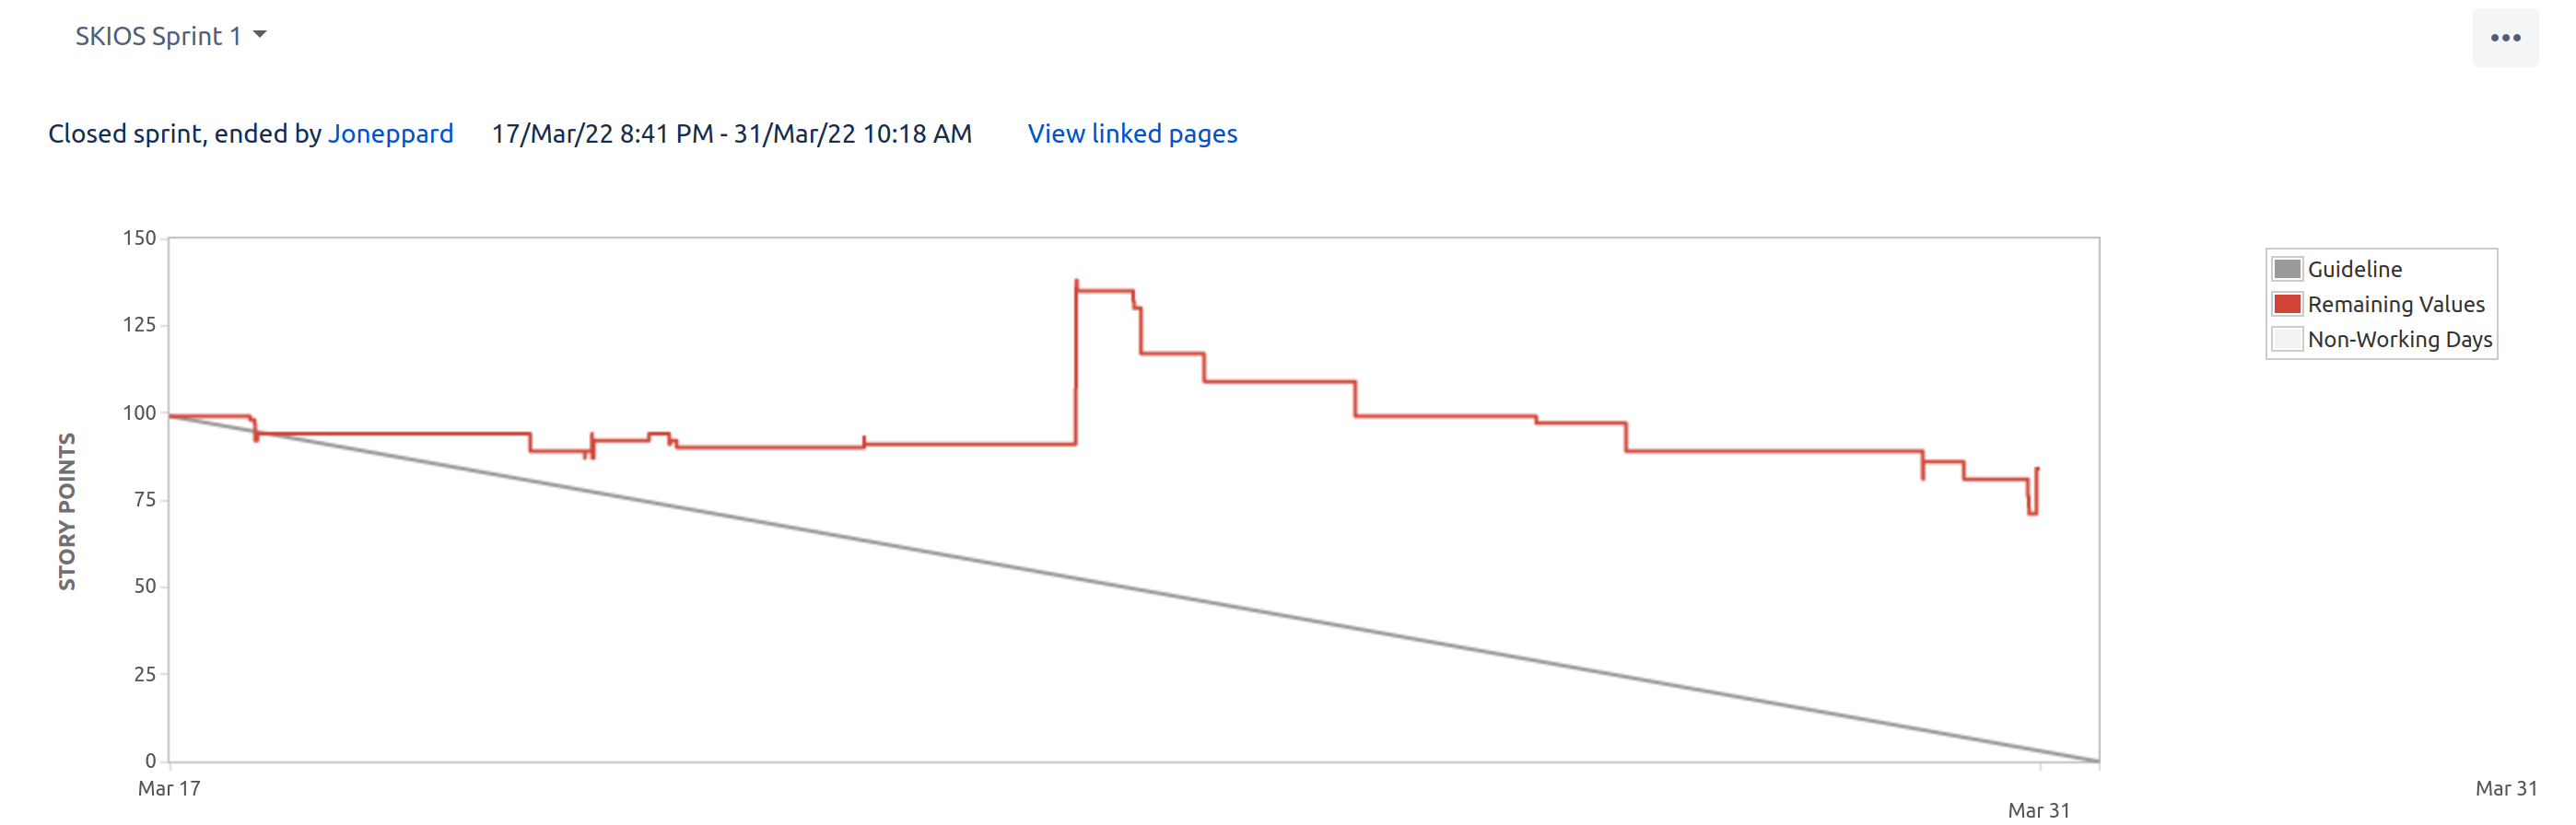
\includegraphics[width=\linewidth]{SKIOS-Sprint-1-Brundown-Diagram.png}
    \caption{Brundown-Chart zu Sprint 1}
    \label{fig:SKIOS-Sprint-1-Brundown}
\end{figure}

Unteranderem wurde in der Retrospektive daraufhin festgehalten, 
dass sich die Kapazitäten zwischen den einzelnen Teammitgliedern sehr stark unterschieden.
Damit genauer geplant werden kann, wurde im Confluence eine Seite zur Kapazitätsschätzungen eingerichtet. 
Dabei handelt es sich um eine Tabelle, inder jedes Teammitglied in Storypoints die eigene Kapazität einschätzen konnte.
Diese wurde wie in Abbildung~\ref{fig:Capacitytable} erstellt. 

\begin{figure}[h]
    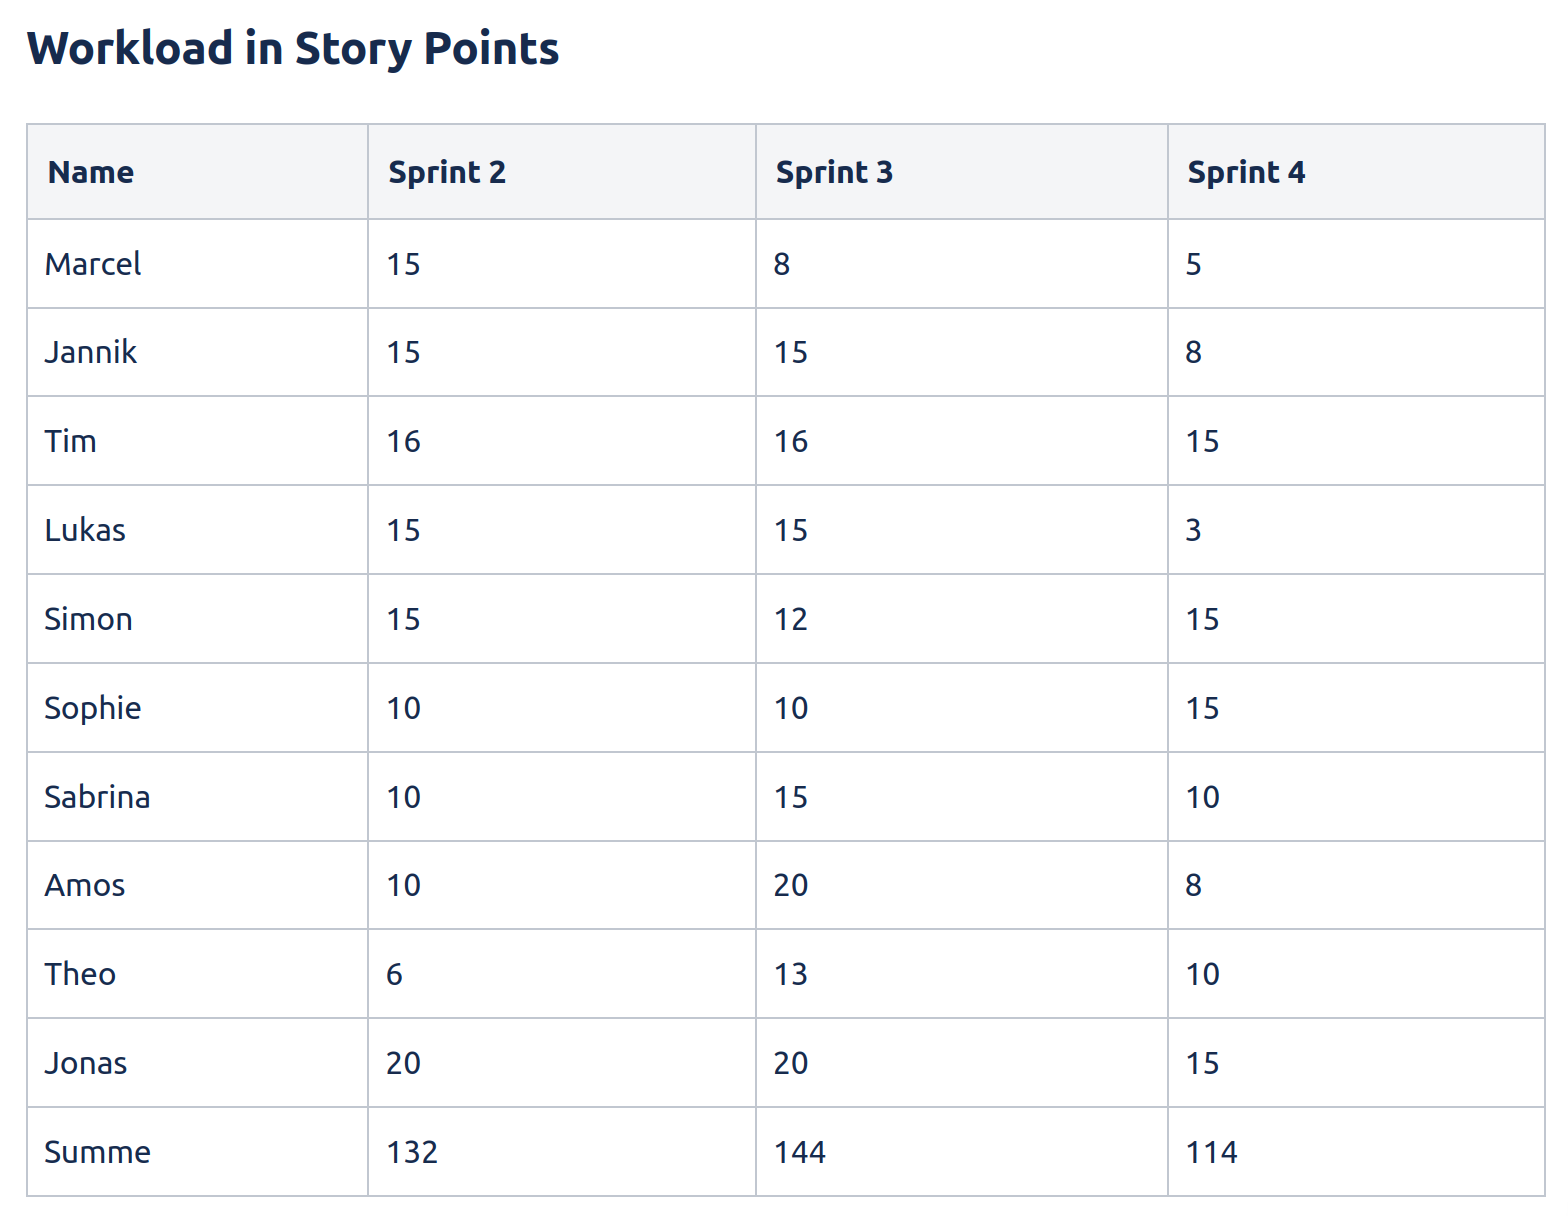
\includegraphics[width=\linewidth]{SKIOS-Capacity-Esitmates.png}
    \caption{Kapazitätschätzungen der Teammitglieder}
    \label{fig:Capacitytable}
\end{figure}

Mit einer besseren Kapazitätsschätzung konnte im nächsten Sprint, dann auch alle vorgenommenen Tickets abgeschlossen werden (vgl. Abbildung~\ref{fig:SKIOS-Sprint-2-Burndown}).
Es war möglich zumindest vorhersehbare Ereignisse, die die Kapazität einzelner start einschränken, abzufangen.

\begin{figure}[h]
    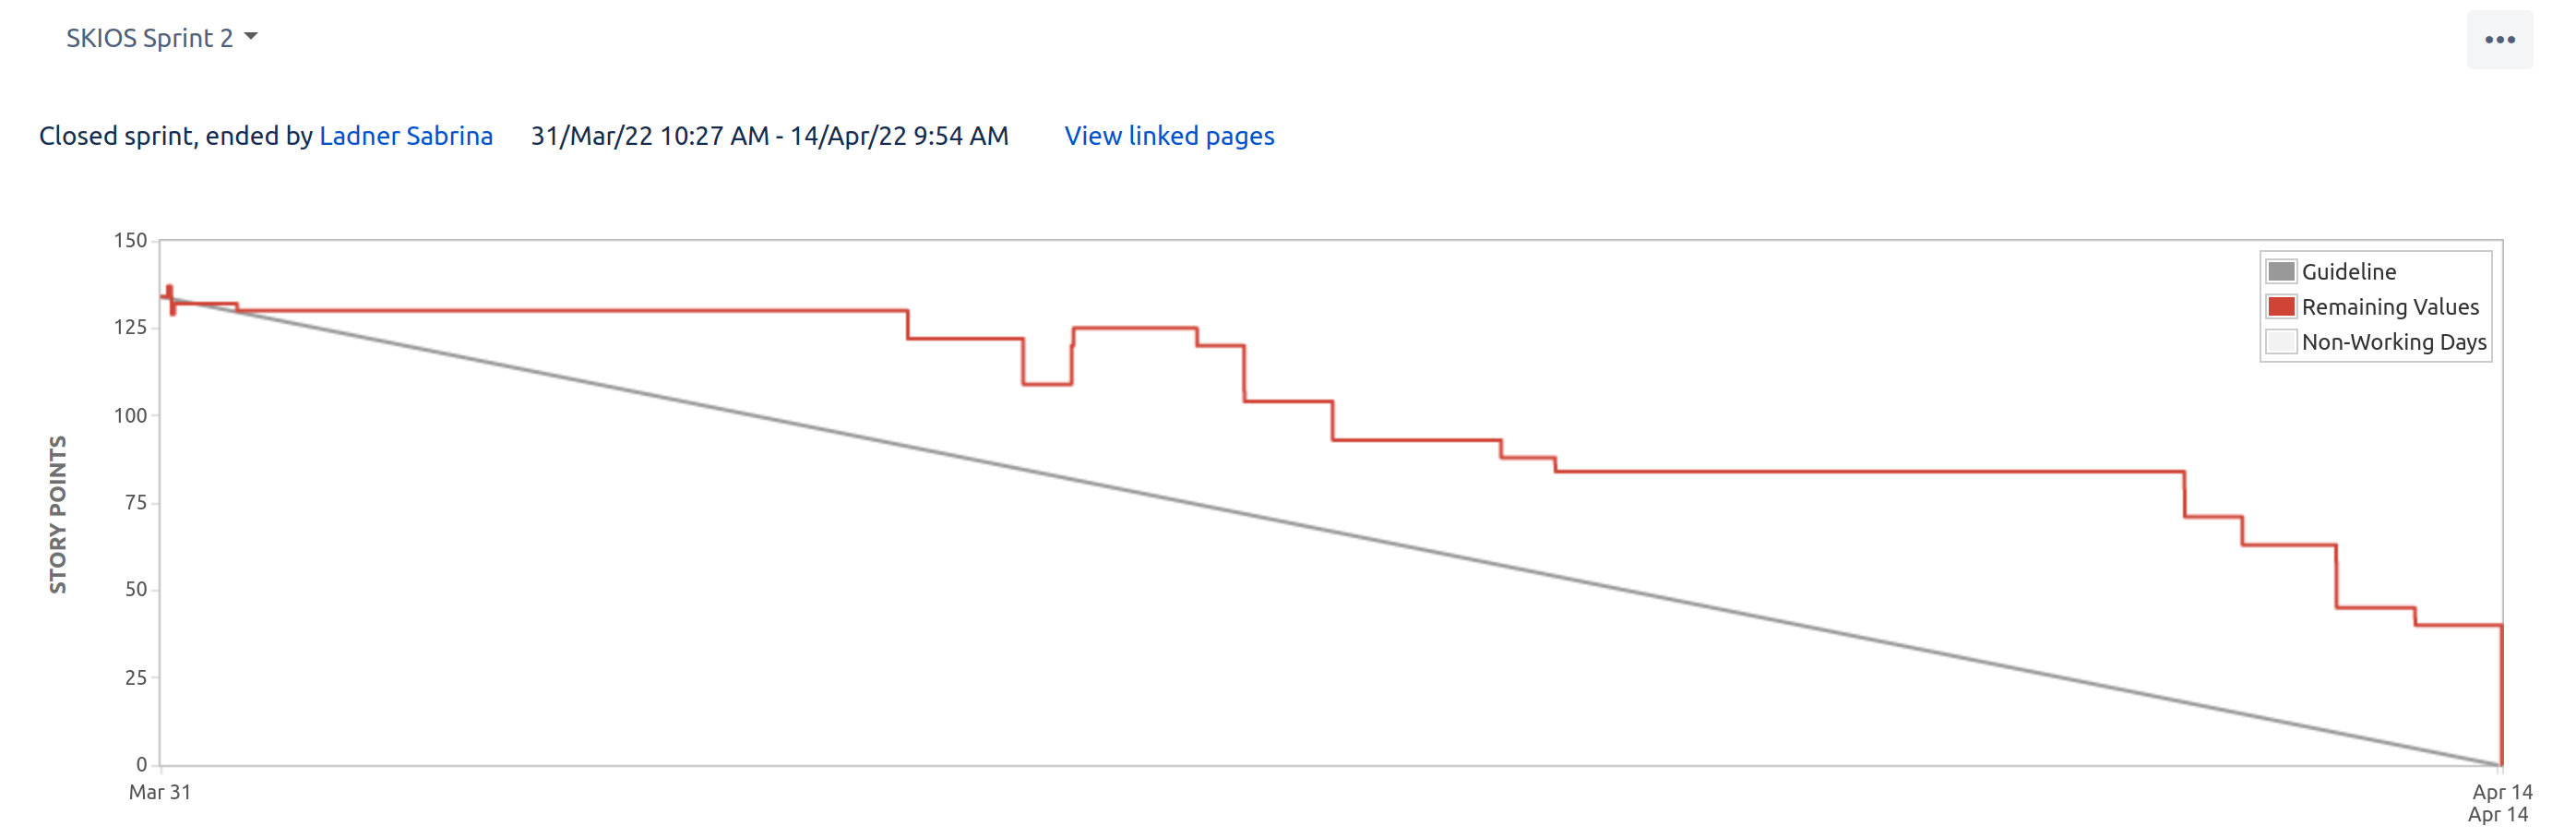
\includegraphics[width=\linewidth]{SKIOS-Sprint-2-Brundown-Diagram.png}
    \caption{Burndown-Chart zu Sprint 2}
    \label{fig:SKIOS-Sprint-2-Burndown}
\end{figure}

\todo{Änderungen des Ablaufes erläutern und analysieren}
\section{Personenbeiträge}
(Zusammenfassung genau beschrieben in den jeweiligen Tickets der Sprints)
